%系统安装,简单的介绍了安装准备事项,安装时的注意事项等
%Author:wgzhao,wgzhao@redflag-linux.com

\section{系统安装}
\begin{frame}[shrink]{Outline}
	\tableofcontents[currentsection]
\end{frame}


%\begin{frame}[t]{Asianux Server 3 安装}
%\begin{columns}
%\column[T]{.5\textwidth}
%	
\includegraphics[scale=.3]{images/axs3-install/box}
%\column[t]{.4\textwidth}
%	\begin{description}
%	\item[kernel] 2.6.18
%	\item [gcc] 4.1.2
%	\item [gtk2] 2.10.4
%	\item [openssh] 4.3p2
%	\item [perl] 5.8.8
%	\item [python] 2.4.3
%	\item [php] 5.1.6	
%	\end{description}
%\end{columns}
%\end{frame}

\subsection{安装前准备}

\begin{frame}{安装前的准备}
\begin{itemize}
\item 原有数据备份
\item 空间规划
\item 多种安装方式

	\begin{itemize}
	\item 光盘直接安装
	\item 硬盘安装,使用iso文件
	\item 网络安装: FTP, HTTP, NFS
	\end{itemize}
\end{itemize}

\end{frame}

\subsection{安装步骤}

\begin{frame}{光盘安装步骤}
\begin{enumerate}
\item BIOS中光驱设置成启动方式
\item 安装方式
	
	\begin{enumerate}
	\item 图形安装
	\item 文本安装
	\end{enumerate}
\item 安装步骤

	\begin{enumerate}
	\item 分区处理
	\item 交换分区 swap 1\textasciitilde{}2倍内存值
	\item 根目录 /
	\item 不同目录安装到不同分区
	\end{enumerate}
\end{enumerate}

\end{frame}


\begin{frame}{光盘启动界面}

\begin{columns}[t]
	\column[t]{.5\textwidth}
	\begin{exampleblock}{插入系统光盘后启动}
	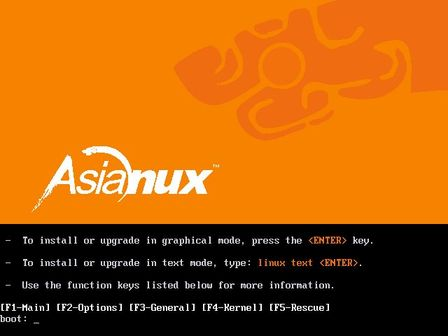
\includegraphics[width=6cm]{images/axs3-install/boot}
	\end{exampleblock}
	
	\pause
	\column[t]{.4\textwidth}
		\begin{exampleblock}{常用的安装内核参数}
			\begin{itemize}
			\item text
			\item acpi=off noapic
			\item dd
			\item rescue
			\end{itemize}
    \end{exampleblock}
\end{columns}
\end{frame}


\begin{frame}{介质检查}

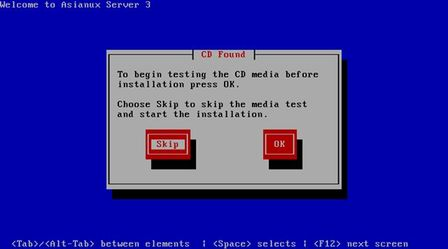
\includegraphics[width=.5\textwidth]{images/axs3-install/disc-check}

\alert{一般可以直接跳过,除非你想确定介质是否完整}

\end{frame}


\begin{frame}{语言选择}
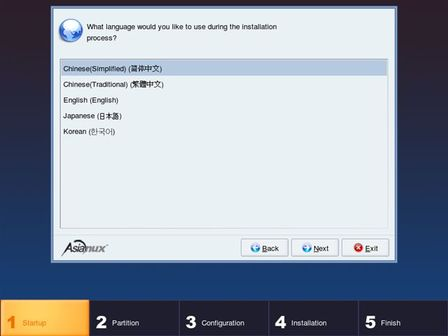
\includegraphics[width=.5\textwidth]{images/axs3-install/lang-choose}
\end{frame}


\begin{frame}{许可协议}

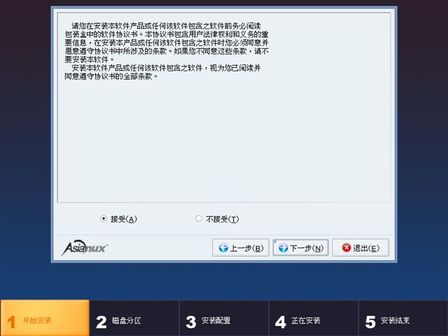
\includegraphics[width=.5\textwidth]{images/axs3-install/eula}
\end{frame}

\begin{frame}{设置键盘}

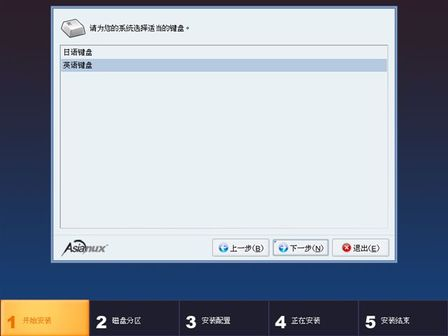
\includegraphics[width=.5\textwidth]{images/axs3-install/keyboard}

\end{frame}
\begin{frame}{选择分区方式}

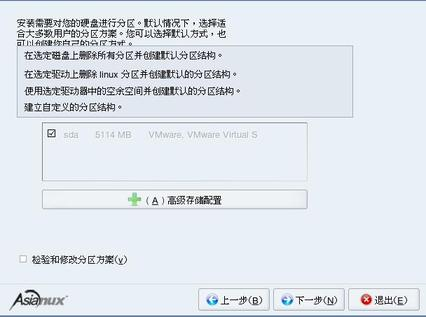
\includegraphics[width=.5\textwidth]{images/axs3-install/partition-method}
\end{frame}

\begin{frame}{设置分区}

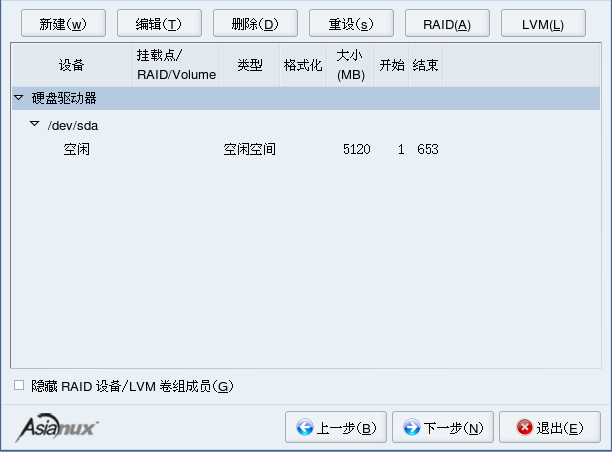
\includegraphics[height=.5\textheight]{images/axs3-install/partition-setup}

\pause
\begin{description}
	\item[/boot] 	 			 \small{引导分区,存放内核以及引导文件}
	\item [/]	根分区,存放操作系统文件
	\item [swap] 交换分区,无挂载点,用作虚拟内存
	\item [/home] 用户分区,存放除root外的用户文件
\end{description}

\end{frame}

\begin{frame}{Linux磁盘及分区识别}
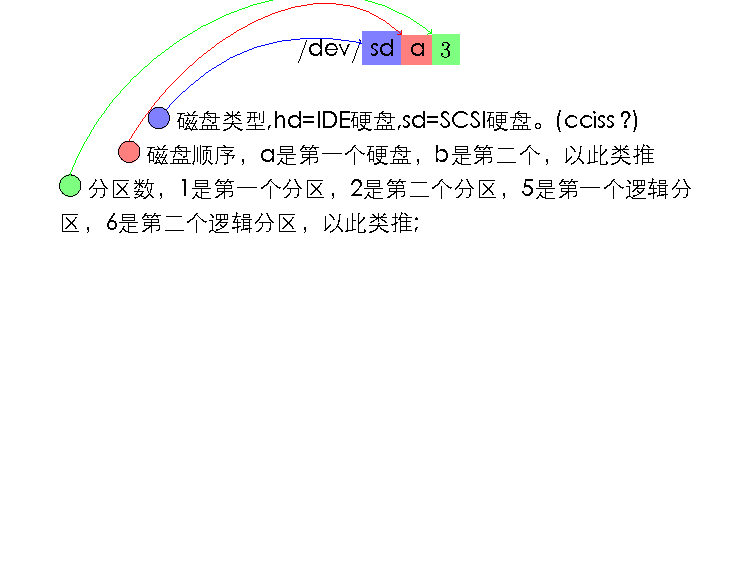
\includegraphics[scale=.8]{disk}
\end{frame}



\begin{frame}[shrink=5]{添加新分区}
	\begin{columns}[t]
		\column{.5\textwidth}
		\begin{exampleblock}{}
			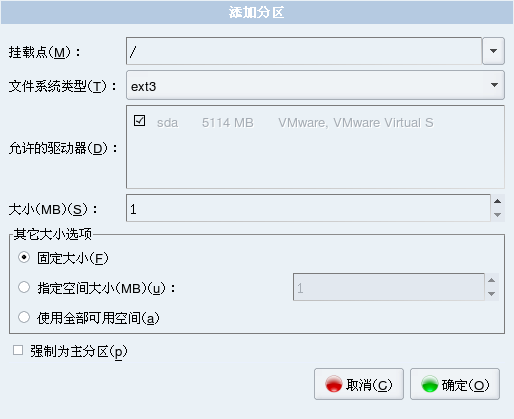
\includegraphics[scale=.35]{images/axs3-install/parition-add}%
		\end{exampleblock}
		
		
		\column[t]{.4\textwidth}
			\begin{exampleblock}{说明}
			\begin{description}
				\item [挂载点] \small{和分区对应起来的目录 /,/home,/var,/etc \ldots}
				\item [文件系统类型] \small{默认使用ext3,交换分区使用swap类型}
				\item [大小] \small{一般情况下/boot 100M,/ 20G,swap 内存的1~2倍}
			\end{description}
			\end{exampleblock}
		\end{columns}

\end{frame}


\begin{frame}{设置根用户口令}

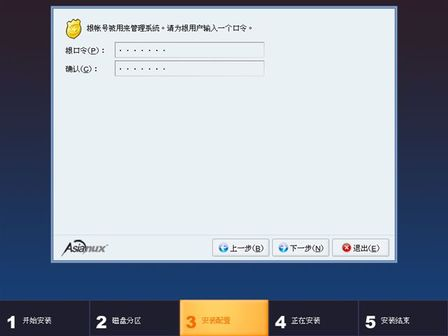
\includegraphics[width=.7\textwidth]{images/axs3-install/password}

\alert{账号是root,这是系统缺省安装后,唯一一个可以登陆的账号}

\end{frame}
\begin{frame}{设置显卡及分辨率}

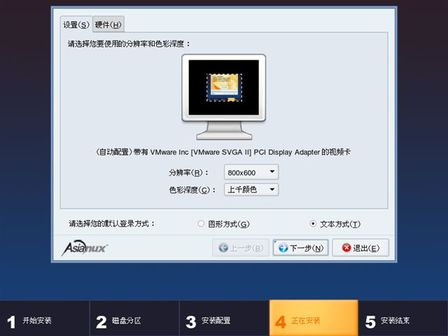
\includegraphics[width=.5\textwidth]{images/axs3-install/resolution}

\end{frame}
\begin{frame}{登录后的界面}

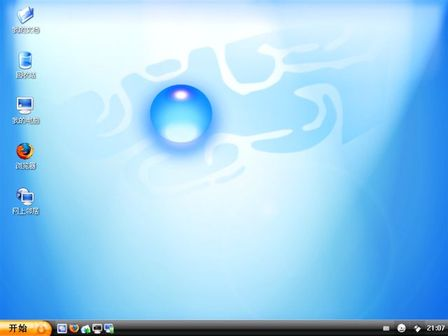
\includegraphics[width=.5\textwidth]{images/axs3-install/desktop}
\end{frame}

